\chapter{Support vector machines}

\section{Introduzione}
Le support vector machines permettono di trovare l'iperpiano ottimo che separa i training data. 
Il training nelle SVM avviene in modalità online.
Si nota come fino ad ora c'era una grande variabilit\`a nell'iperpiano che il classificatore lineare trova cominciando da diversi punti nell'iperspazio.
Inoltre quando i dati non sono linearmente separabili questa variabilit\`a aumenta grandemente.

	\subsection{Considerazioni su perceptron e gradient descent}
	Come visto il perceptron se i dati sono linearmente separabili trova un qualche iperpiano che li separa, che non \`e necessariamente il migliore, altrimenti continuer\`a ad aggiustarsi iterando attraverso gli esempi e l'iperpiano dipender\`a dall'ultimo esempio visto.
	Il gradient descent invece trova l'iperpiano che minimizza $loss+regularization$ in entrambi i casi.
	
	\subsection{Idea delle support vector machines}
	Le support vector machines cercano di trovare il migliore iperpiano separa i dati. 
	Per migliore intendiamo quello con il margine pi\`u grande.
	Per definirlo vengono introdotti i margini di un iperpiano.

\section{Margini}
I margini di un iperpiano sono la distanza dal punto pi\`u vicino.
Maggiore il margine meglio l'iperpiano separa le classi.
Il fatto che il modello trovato da una SVM ha il maggior margine possibile aumenta l'abilit\`a di generalizzazione del modello.

	\subsection{Support vectors}
	I support vectors sono i data points pi\`u vicini al margine che separa i dati.
	Per $n$ dimensioni ci saranno almeno $n+1$ support vectors.
	Il fatto di massimizzare il margine implica che solamente i support vector contano a tempo di inferenza e tutti gli altri punti possono essere ignorati, perch\`e tramite quelli \`e definito l'iperpiano.
	
	\subsection{Calcolare il margine}
	Il margine pu\`o essere pertanto calcolato come la distanza dal support vector.
	La distanza di un punto $x$ da un'iperpiano viene calcolata come $d(x) = \frac{wx+b}{||w||}$.
	Il margine viene calcolato pertanto come $\frac{c}{||w||}$, dove $c$ \`e la traslazione dell'iperpiano in modo che la sua distanza dal support vector sia $0$.
	Si nota come scalando il vettore dei pesi $w$ la distanza dall'iperpiano rimane la stessa.
	Inoltre essendo $c$ e $w$ strettamente correlati si pu\`o assumere $c=1$ sempre.
	
	\begin{figure}
		\centering
		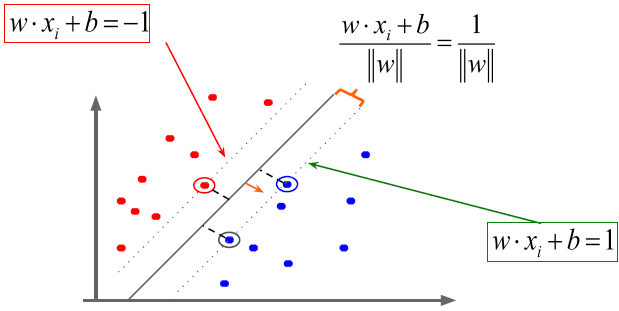
\includegraphics[width=0.6\linewidth]{imgs/chapter10/img0}
		\caption{Misurazione del margine}
		\label{fig:chapter10-00}
	\end{figure}

\section{Problema di ottimizzazione}
Si vuole pertanto massimizzare il margine ma classificando correttamente ogni esempio.
$$argmax(margin(w,b))\qquad\land\qquad y_i(wx_i + b) \ge 1 \forall i$$
A parole: con la prima equazione indichiamo che vogliamo trovare il margine massimo, con la seconda indichiamo che vogliamo che tutti i punti siano al di fuori del margine (o sul margine).
L'errore viene tenuto basso dal fatto di avere tutti i data point al di fuori dal margine come stabilito dalla seconda equazione.

	\subsection{Massimizzare il margine}
	Per massimizzare il margine intendiamo trovare
	$$max_{w,b}\dfrac{1}{||w||}$$
	Tenendo d'occhio l'errore.
	Massimizzare il margine \`e equivalente a minimizzare la normale dei pesi:
	$$min_{w,b}||w||$$
	Si vuole pertanto avere il vettore di pesi minore possibile $w$.
	$c=1$ \`e un'assunzione che si fa in quanto altrimenti si starebbe imparando una versione scalata dello stesso problema in quanto per ogni support vector $c = w\cdot x_i +b = 1$.
	In realt\`a si tenta di minimizzare:
	$$||w||^2 = \sum\limits_{j\in I}|w_j|^2$$
	Soggetto a $y_i(wx_i+b) \ge 1$.
	Questo \`e lo stesso problema con il vantaggio che \`e una funzione convessa con lo stesso minimo della norma di $w$.
	In questo modo diventa un problema di ottimizzazione quadratica, di risoluzione semplice.
	Utilizzando questo regolarizzatore diventa difficile utilizzare SVM per fare feature selection, perché per ignorare una feature, il suo peso deve essere 0, ma il regolarizzatore utilizzato penalizza valori grandi, e difficilmente avremo pesi che raggiungono 0.

\section{Soft margin classification}
La soft margin classification permette di usare SVM quando i punti non sono linearmente separabili.
Quando qualche dato non \`e linearmente separabile non si riescono a soddisfare i due costraint necessari per train le SVM e pertanto si necessita di modificare la funzione obiettivo.
Per farlo si permette al modello di fare delle predizione sbagliate, ma si aggiunge alla funzione obiettivo una penalit\`a per ogni esempio classificato erroneamente.
Queste sono dette slack penalties e sono usate per ottenere un modello che accetta con una certa tolleranza errori di classificazione.
La funzione da ottimizzare diventa pertanto:
$$\min_{w,b}||w||^2+\mathcal{C}\sum_i\zeta_i\qquad subject\ to\qquad y_i(wx_i+b)\ge 1 -\zeta_i\forall i, \zeta_i \ge 0 \forall i$$
Si nota come $\zeta_i$ sono le slack variables e se ne trova una per ogni esempio nel dataset e sono utilizzate per correggere classificazioni sbagliate, ma poi il loro peso \`e aggiunto alla funzione obiettivo.
Si vuole pertanto trovare un trade-off tra minimizzare il quadrato della norma, quindi le dimension del margine, di $w$ e il valore di penalit\`a dato dalla slack variable, quindi gli errori che facciamo.
La somma di $\zeta_i$ misura la tolleranza agli errori.
Si nota come:
\begin{multicols}{2}
	\begin{itemize}
		\item Piccoli valori di $\mathcal{C}$ permettono pi\`u errori che consistono in un margine pi\`u grande. 
		Con un margine troppo grande andremo in underfitting.
		\item Grandi valori di $\mathcal{C}$ danno agli errori di classificazione pi\`u peso restringendo il margine. 
		Con un margine troppo piccolo andremo in overfitting.
		\item $\mathcal{C} = \infty$ impone tutti i costraint e riduce a un hard margin.
	\end{itemize}
\end{multicols}
I valori di $\zeta_i$ sono imparati insieme a $w$ e $b$.
$\mathcal{C}$ \`e un iperparametro per controllare l'overfitting, noi siamo interessati a trovare il miglior $\mathcal{C}$ per il training set.
Si nota come questo \`e ancora un problema di ottimizzazione quadratica con costraint lineari, ma il numero di calcoli con un training set medio grande \`e molto elevato.
\begin{figure}
	\centering
	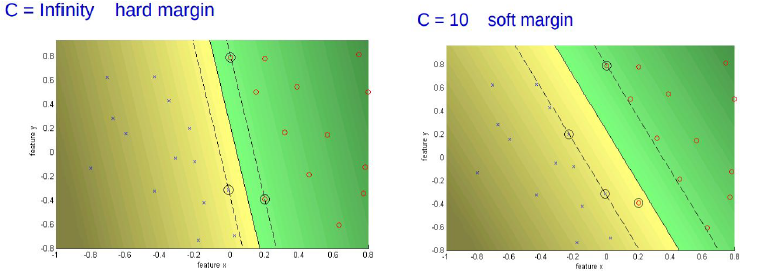
\includegraphics[width=0.6\linewidth]{imgs/chapter10/img1}
	\caption{Il significato dell'iperparametro $\mathcal{C}$}
	\label{fig:chapter10-01}
\end{figure}

	\subsection{Risolvere il problema delle SVM}
	Data la soluzione ottimale $(w,b)$ si pu\`o calcolare la slack penalty per ogni punto.
	Per tutti gli esempi correttamente classificati al di fuori del margine (o sul margine), dunque se vale $y_i(w \cdot x_i+b) \ge 1$, il valore dovr\`a essere $0$.
	Per gli esempi correttamente classificati all'interno del margine sar\`a la distanza dal punto e la linea del margine, che pu\`o essere calcolata come $1-(valore\ della\ funzione\ di\ decision)$, un valore compreso tra $0$ e $1$, in particolare:
	$$\zeta_i = 1 - y_i(w \cdot x_i+b)$$
	I dati classificati con errore il valore \`e dato dalla somma della distanza dall'iperpiano pi\`u la distanza dal margine, con la stessa formula come nel caso precedente.
	Si riassume la formula in:
	$$\zeta_i = \max(0,1-yy')$$	
	Che si nota che \`e la hinge loss function.
	Trasformando la funzione obiettivo di un SVM in una funzione di hinge loss si trasforma il problema in uncostrained in quanto entrami i costraint sono tenuti in considerazione dalla funzione.
	La nuova funzione obiettivo pertanto sar\`a:
	$$\min_{w,b}||w||^2+\mathcal{C}\sum_i\max(0,1-y_i(wx_i+b))$$
	Che pu\`o essere considerata come un problema di gradient descent con Hinge loss function e regolarizzatore $||w||^2$.
	La soluzione a questo problema trova pertanto l'iperpiano con il margine pi\`u grande possible permettendo un soft margin. 
	Il vantaggio di utilizzare soft-margin SVM rispetto a qulle hard-margin \`e che con quelle soft-margin abbiamo la garanzia di trovare una soluzione anche nel caso i dati non siano linearmente separabili, mentre in quelle hard-margin la regione all'interno dei margini \`e sempre vuota.

\section{Dati non linearmente separabile}
Per separare i dati non linearmente separabili si possono utilizzare spazi con dimensioni maggiori.
Prima si tentava di risolvere un problema di ottimizzazione quadratica soggetto a un'insieme di costraint lineari.
Questo \`e il problema primario delle SVM.
Si pu\`o riscrivere questo problema nella forma di un dual problem.
Si noti come i problemi di ottimizzazione quadratica sono una classe ben conosciuta di problemi di programmazione per cui esistono diversi algoritmi non banali.
Una possibile soluzione coinvolge costruire un dual problem dove un moltiplicatore di Lagrange $a_i$ \`e associato con ogni costraint di ineguaglianza nel problema originario.
Si deve pertanto trovare $a_1,\dots,a_n$ tale che:
$$Q(a) = \sum a_i - \frac{1}{2}\sum\sum a_ia_jy_iy_jx_i^Tx_j$$
\`e massimizzato e $\sum a_iy_i = 0$ e $a_i\ge 0\forall a_i$.
Il problema \`e pertanto massimizzare $Q(a)$, un problema di ottimizzazione quadratico con un paio di costraint lineari.
Un buon risolutore scalabile \`e $SM)$.
Una volta risolto il dual problem e ottenuto tutti i valori di $a_i$ posso computare $w$ e $b$:
$$w=\sum a_iy_ix_i$$
$$b = y_k - \sum a_iy_ix^Tx_k$$
Per ogni $a_k>0$.
Pertanto la funzione classificatrice \`e:
$$f(x) = \sum(a_iy_ix_i^Tx)+b$$
Si nota come tutte le $a_i$ degli esempi che non sono support vector hanno valore $0$, pertanto non si necessita di esplicitare $w$ se si conosce $a$.
In quanto $x$ compare solo nel dot product nella funzione di predizione e di ottimizzazione e $a$ \`e nulla per ogni esempio non support vector il loro impatto \`e nullo: una volta trainata la funzione di predizione pu\`o mantenere solo i support vector risparmiando memoria.

	\subsection{Soft margin classifier}
	Il dual problem \`e simile nel caso del soft margin classifier: si deve trovare $a_i,\dots, a_n$ tali che:
	\begin{itemize}
		\item Massimizzano $Q(a) = \sum a_i-\frac{1}{2}\sum\sum a_ia_jy_iy_jx_i^Tx_j$.
		\item $\sum a_iy_i = 0$
		\item $0\le a_i\le \mathcal{C}\forall a_i$
	\end{itemize}
	Si nota come $x_i$ con non zero $a_i$ sono support vectors.
	Pertanto la predizione dipende solo dai support vectors.
	Con entrambi gli approcci si impara un iperpiano che separa i datapoints e in entrambi solo i data points rilevanti per la prediction function sono i support vector.
	
	\subsection{Identificare i support vector}
	I support vector sono identificati dagli algoritmi di ottimizzazione quadratica come i training point con non zero lagrangian multipliers $a_i$ in quanto i training point appaiono unicamente all'interno prodotti interni, pertanto non li necessito ma solo i loro dot-product.
	
	\subsection{Utilizzo di SVM in maniera non lineare}
	Se i dati non sono linearmente separabili si possono portare a uno spazio a dimensioni maggiori rendendoli linearmente separabili.
	Lo spazio delle features originali pu\`o essere sempre mappato a uno spazio di features con dimensione maggiore dove il training set \`e separabile.
	Il problema di ottimizzazione e la funzione di predizione dipendono solo dal prodotto dei vettori di features degli esempi.
	Il classificatore lineare dipende sul prodotto interno di questi vettori:
	$$K_{linear}(x_i,x_j) = x_i^Tx_j$$
	Se ogni data point \`e mappato in uno spazio con maggiore dimensione attraverso una qualche trasformazione $\phi:x\rightarrow\phi(x)$, il prodotto interno diventa:
	$$K_{for\ function\ \phi}(x_i,x_J)= \phi(x_i)^T\phi(x_j)$$

		\subsubsection{Kernel function}
		Una kernel function \`e una funzione equivalente a un prodotto interno in uno spazio di features.
		In generale non si \`e interessati a $\phi$ ma alla funzione kernel in quanto mappa i dati a uno spazio a maggiore dimensione implicitamente \ref{fig:chapter10-02}.
		
		\begin{figure}
			\centering
			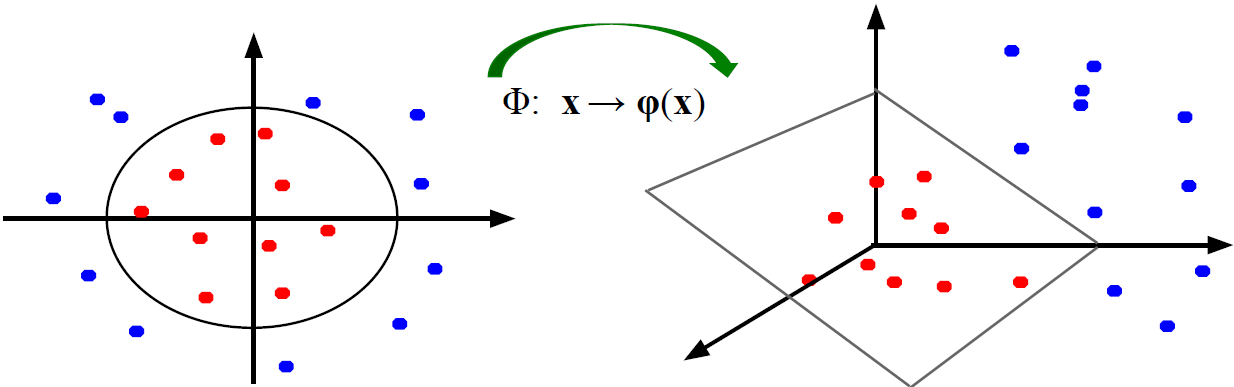
\includegraphics[width=0.6\linewidth]{imgs/chapter10/img2}
			\caption{Kernel function}
			\label{fig:chapter10-02}
		\end{figure}
		
		Ogni kernel ha un iperparametro a parte la lineare.
		\begin{itemize}
			\item Linear: $K(x_i,x_j) = x_i^Tx_j$
			\item Polinomial of power $p$: $K(x_i, x_j) = (1+x_i^Tx_j)^p$.
			\item Gaussian o radial-basis: $K(x_i, x_j) = e^{\frac{|x_i - x_j|^2}{2\sigma^2}}$.
			In questo caso ogni punto \`e mappato a una funzione gaussiana e $\phi(x)$ ha infinite dimensioni.
			La combinazione delle funzioni per i support vectors \`e il separatore.
		\end{itemize}
		Lo spazio a maggiore dimensioni ha una dimensionalit\`a $d$ intrinseca ma il separatore lineare in esso corrisponde a un separatore non lineare nello spazio originale.
		
		\paragraph{Teorema di Mercer}
		\begin{itemize}
			\item Ogni funzione simmetrica semi positiva \`e un kernel.
			\item Le funzioni semi-positive simmetriche corrispondono a una matrice di Gram semi-positiva definita
		\end{itemize}

		\subsubsection{Soluzione del problema scelto il kernel}
		Una volta scelto il kernel il problema diventa trovare $a_1,\dots,a_n$ tali che:
		\begin{itemize}
			\item Massimizzano $Q(a) = \sum a_i-\frac{1}{2}\sum\sum a_ia_jy_iy_jK(x_i,x_j)$.
			\item $\sum a_iy_i = 0$
			\item $a_i\ge 0\forall a_i$
		\end{itemize}
		La soluzione \`e:
		$$f(x) = \sum a_iy_iK(x_i,x)+b$$
		La tecnica di ottimizzazione per $a_i$ rimane la stessa.
		Si nota come risolvendo il dual problem con il kernel giusto si risolve il problema SVM portando i dati in uno spazio a dimensione maggiore in cui \`e linearmente separabile e non perdiamo informazioni.
